\documentclass[a4paper,11pt]{article}

% packages
\usepackage{array}
\usepackage{tabularx}
\usepackage{booktabs}
\usepackage{graphicx}
\usepackage{framed}
\usepackage{comment} % comment multiple lines
\usepackage{spverbatim} % pasting large amounts of texts such as SQL code, and more
\usepackage{alltt}
\usepackage{float}
\usepackage{url} % URLs used for 
\usepackage{fancyhdr}
\usepackage[utf8]{inputenc} % Use UTF 8. This allows æ, ø, å

% commands
\newcommand{\ra}[1]{\renewcommand{\arraystretch}{#1}} % custom command used for tables
\newcommand{\specialcell}[1]{\begin{tabular}{@{}c@{}#1\end{tabular}}}
\newcommand{\CS}{C\nolinebreak\hspace{-.05em}\raisebox{.6ex}{\tiny\bf \#}}

% define the author and title for frontpage
\author{
	\textbf{Oz}\\
	\textbf{Group 6}\\
	Nicolai Ditlev Krogh Krüger\\
	Philip Rasmussen\\
	Morten Drescher Salling\\
	Michael Søby Andersen\\
	Claus Lindquist Henriksen
	}
\title{BSUP, Spring 2013}
\pagestyle{fancy}
\begin{document}
\maketitle
\tableofcontents
\newpage

% Inputs
\addcontentsline{toc}{section}{\hspace{17pt}Abstract} % Adds to the Table of contents
\section*{Abstract}
\rhead{\textit{ABSTRACT}} % Set header
\lhead{} % Set header
% 0.5 page, not part of report itself

When a software project runs amok and gets delayed rarely anyone benefits from it.
When it happens, it is crucial to know which selection of methods to apply in order to get the project back on track and end as close to the deadline as possible.
In this paper we will consider a derailed project of small size, which is relatively simple and run by a group of about five members.
We consider multiple development, planning, and estimation methods, assessing their benefits and drawbacks if they were applied to a project of the considered type.

Through use of Planning Poker, a variant of SCRUM, a dependency network diagram, peer reviewing, and a custom method for planning meetings, we show how a project similar the one described may be helped back on track.

\newpage
\fancyhead[R]{\leftmark}
\fancyhead[L]{\rightmark}

\section{Introduction}
% 0.5 page
This paper was written for the course `System Development and Project Organization, BSUP' at IT-University of Copenhagen in the spring 2013.

In almost every software development project some degree of planning and application of development methods are needed - a need which increases with the size of the project group, the project size, and critical factors \cite[p. 134]{ac}. For larger projects the right choices of planning and development methods are essential for meeting the requirements and deadlines.

When a project goes off its tracks, however, it can be difficult to get it back. First one must review and adjust the chosen methods used for the project to avoid further derail from happening, which involves discovering why the project derailed in the first place.
Once the work process has been adjusted, changes to the project plan are also necessary: If the right adjustments are not made, the project is unlikely to be finished with desirable quality within the designated time frame.

In this paper we consider a such derailed project.
In the first part we will empirically describe the events which lead up to the derailing, identifying the cause of the problems. In the second part we will attempt to identify the proper methods for getting the project back on track and describe the observed results of applying these. At last we will discuss and conclude how well we managed to `rescue' the project based on the resulting quality, and finally we will give a perspective of our findings.
\section{Problem statement}
% 1 page
We have a project that has gone off its rails. How do we get it back on track, meeting both the requirements and the deadline?
\begin{itemize}
\item Which planning tools can we use to our benefit?
\item Which selection of development methods is able to boost our productivity with minimum overhead from using the methods themselves?
\item Which methods should we use to maintain and measure quality?
\item How well does application of these methods allow us to recover our project, as determined from the quality of the final product?
\end{itemize}
We would also like to discuss when we think the project derailed, why it did so, and which measurements we could have taken to prevent it.
\newpage
\section{Problem Analysis}
The derailed project we considered was our 2\textsuperscript{nd} year project, which was divided into two parts. In the first part of the project we cooperated with a Singaporean group (SMU) over five weeks to build a rental system. We built the server part of the system, while the Singaporean group simultaneously developed the client to consume our services.

We had chosen to write the server using F\#, a new language we were learning in parallel with the project. We thought it would be an excellent opportunity to see how it performed when applied to a real project.
Working with the .NET platform, we had also decided to use WCF to publish our services, something we had experience with from the previous semester. Previously this had been SOAP, but we saw several benefits from designing the API RESTfully, although this would be another new area to explore.
Having talked with our tutor, we were advised to add a thin layer of C\# code between the WCF layer and our backend code in F\#, since F\# did not play that well with WCF yet. The sole purpose of the C\# code would be to pass on requests to the backend and give back the results received.
At last we also decided against using the ADO.NET Entity Framework and instead write our own database communication code to maximize freedom and transparency of the persistence layer.
We knew it would be a lot of work, but decided to do all of it anyway, even though the collaboration also would be a new experience to us. This decision was probably the main source of later problems. \textbf{[ TODO: Write something about the uncertainties when working with new stuff, all the unknown factors ]}

As development methodology we chose not to use SCRUM, since most of the group based on previous experience felt that we would spend more time to set it up than we would gain from using it. Also our individual time schedules and short time frame made it difficult to set up sprints of effective lengths, where everybody would be able to participate. We did not anticipate how much the lack of detailed planning affected our work, but expected that the time we saved would exceed the extra spent from not planning.

After a preparation period of about a month, the collaboration was about to begin, at which point no work had been performed yet. The requirements of the system were to be negotiated with SMU, and so were the interface of our part of the system.

A week after the preparations had begun, the requirements were in place and the first half of a very detailed API documentation were ready, although documentation of the full API had been agreed to be done. For consistency reasons a single person had been designated to write the document, but since we did not have experience writing such documents, the extent came as a surprise.

With only four weeks left of the collaboration, SMU needed our server to provide functionality soon, and the part of the API already documented was agreed to be implemented and running by the end of the week. Since we did not use SCRUM, time was not spend estimating the extent of the work in detail. Time was short, but with hard work we estimated the deadline to be possible.
Had we used familiar tools and languages, the estimates would probably had been correct, but none of us had taken the many new technologies into account.

Without planning our overview also got lost: Layers of the functionality was distributed among the team members, but time was not spent in the group talking about the overall architecture.

By the end of the week, all members had experienced problems to some extent because of the new technology, and the code were by no means ready for deployment.
Problems figuring out how to configure WCF properly arose; it turned into a bigger task than anticipated getting the C\# layer and the frontend of the F\# backend to communicate; and the F\# code, its structure, and its internal communication, suffered from our lacking knowledge of the language and how to built generic, modular systems using it.

At the beginning of next week the WCF layer was not finished yet, and though the backend seemed to be ready, we could not deploy. The structural problems started to show, and after an extensive code review it became apparent that refactoring would be needed.
SMU began asking for a schedule of when each server feature would be implemented, which they were given, although the dates were set arbitrarily as they needed to in order for all functionality to be fitted into the schedule. Looking back, this schedule was highly unrealistic, but we deemed it possible, probably because no estimations of each required feature had been made.

Thursday, four days over deadline, the first part of the service was deemed ready for deployment, at which point some refactoring also had been made. Thursday was spent deploying the system, which turned out to both be missing agreed functionality and containing severe bugs. The system was deployed, but parts of the system were not functional and essential concurrency-controlling code had to be commented out in order for the system to be functional.

The second half of the web service API was ready the next Monday where it was accepted by SMU. Next we carried out refactorizations, which had shown to be essential, and planned our activities for the easter holidays, in which the team would not be able to assemble. After the holidays only a week was left of the collaboration, which we reserved for bug fixing and deployment. The layers of functionality was split between the team members to be developed individually during the holidays.

When the holidays ended, the WCF layer had been refactored completely, and although it was meant to be thin, this was by no means the case. It was missing almost all functionality that should had been implemented during the holidays, and so were the case for many other layers of planned functionality.
Not all problems which had shown during the deployment of the first system part had been fixed yet, and large parts of the system were still untested.

Our deadline was in just four days, and it all became very hectic with work during both day and night. In the end not all requirements were fulfilled, much code was untested, entire parts of planned functionality had been dropped, and the overall quality of the code was poor. It was frustrating to debug and hence maintain, and the code contained several bugs, which was found during the following days where none of the team members really had the time to fix them.

After SMU had their deadline they asked us if we could give them some reflection on the collaboration, which gave us a chance to reflect on our process as well. We realized how far into the semester we were and how close our own deadline was. We saw how much time you could potentially waste, when you do not prepare properly to a given project, and how this affects the quality of the product. At this point we realized that the project had derailed completely - and something had to be done to get it back on track!
\newpage
\section{Getting back on track}
% 13 pages
Though planning can help structure the collaboration, it can also add quite a bit of overhead. One should therefore carefully select which planning methods to use and the extent of the planning. If you spend too much time on planning, you might not meet the deadline with all requirements satisfied, and if you spend too little time planning, the project might derail further.

In the following sections we will apply project management theory to re-plan the second part of the derailed project. We will discuss alternative development methodologies and pick the ones we believe suits the project the best, reflecting upon our results of doing so where possible.

We will not discuss the technical aspects of the second project part, although we shortly will mention that we have decided to use only languages and technologies well known to the group.
A significant cause of problems in the first part of the project stemmed from the many new tools we had decided to use without reserving the time for unforeseen problems.
In the second part of the project we do not have time to spare for such problems and have therefore decided to play safe by sticking to the well-known.

\subsection{Planning second half}
% 1 page
The best way to get the project back on track is through careful planning. First of all we needed to get an overview of the remaining parts of the project, and then we wanted to carefully structure and plan: What needs to be done?, In what order? and How much time do we have?

We have divided the planning up into four parts.

We start out by looking at the development methods that we want to use. We give a brief introduction to the method, and explain how we applied it, helping the project back on track

After this we describe the estimation methods we use. The estimation methods should help us make accurate estimations. This, in turn, helps us to meet deadline, as most of our estimations should be correct or close to.

Now that we have found out how much time we need, we need to find out how much time we have available. For this we use a couple of methods for planning the time. Those methods are explained, and our usage is analyzed.

As the last, but most important part, we look into how our save of the product has affected the quality. Less time to do roughly the same work must have some effect on quality. This is analyzed.
% !TeX spellcheck = en_US
\subsection{Method of development}
% 3 pages
In the first part of the project, we entirely decided against using SCRUM because the project and its environment did not allow us to perform all practices dictated by SCRUM. The result was an unstructured development process leading to all kinds of problems.
We do like the SCRUM development method, however, and in this part of the project we will attempt to take a more gradual approach to SCRUM. The project and its environment is still not ideal for full SCRUM, but instead of rejecting SCRUM entirely, we will only reject those parts that are not well suited for the project.

A SCRUM activity we have chosen to exclude among others is the Daily SCRUM meeting.
At the Daily SCRUM meeting the development team and the SCRUM-master is updated with progress and set-backs.
We are a small group of only 5 people, however, and we do not have people to fill out all roles used in proper SCRUM, such as product owner and stake holders - we are only able to represent the development team.
As development will be done with the group assembled, we see no need for spending 15 minutes every meeting updating each other, as we already do this ad hoc when we are working.
The API we have defined and the SCRUM backlog should be enough to make the progress visible to all team members. Any problem which may arise during development may be discussed in plenum immediately.

\begin{figure}[t]
  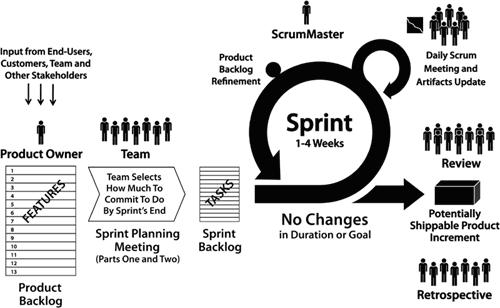
\includegraphics[width=\textwidth]{illustrations/scrum.jpg}
  \caption{An overview of SCRUM and its many activities. Of the displayed practices we have decided to use only the product backlog. Source: [\textit{http://softlinksolutions.com/development\_methodology.aspx}]}
  \label{scrum_picture}
\end{figure}

As just mentioned, we have decided to use a backlog, which is another SCRUM artifact.
The backlog is a prioritized list of items, where each item describes a program feature, often called a `story', possibly with sub-tasks that needs to be completed. Traditionally the product owner defines the order of the items, putting the features he wants implemented first at the top of the list \cite[p. 12]{scrum-org-guide}.
We have chosen to use a backlog as it ensures that the most vital functionality is implemented before less important, nice-to-have features. We will also benefit from producing the backlog itself, as we will be forced into enumerating all features to implement, giving us an overview of the work and ensuring that no big task suddenly pops up later.
Our complete backlog can be viewed in \atref{backlog}.

We have chosen not to divide our project into sprints, even though they are a core foundation of SCRUM.
Sprints are great for projects with longer time spans than ours, as it divides the project into smaller iterations, each producing valuable functionality able to function on its own, making it easier to keep focus.
After every sprint, the SCRUM team do a review, a retrospective, and plan which backlog items to implement during for the next sprint \cite[p. 8]{scrum-org-guide}.
Were we to divide our project into sprints, it would be very short ones, and it would not be worth the overhead from managing sprint backlogs and do reviews and retrospectives.

During a sprint, a SCRUM Task Board artifact is used to maintain overview of the sprint progress. The board is divided into four parts (`not started',`in progress', `to test' and `complete') with each task of the sprint listed under the appropriate section.
When a task is started it is moved from `not started' to `in progress', when a task is finished it is moved to `to test', and when it has passed its tests it is moved to `complete'.
Often a physical board is used so everyone, all the time, is able to keep track of the progress. This however, is only possible if all team members are at the same location, and it may be difficult to do, if the team cannot persist the board between sessions, for instance if the work location changes for each meeting.
For our project we have found a way to deploy a task board with minimum overhead by using a software version, always allowing every team member to keep track of the project wherever they are. Since we do not use sprints, the task board will give an overview of the progress of the whole project and of the individual tasks.\\
Our task board can be viewed in \acref{taskboard}. \textbf{[ TODO: Insert in appendix ]}

The burndown chart in SCRUM (as well as in other measurable environments) is used to monitor the progress of remaining tasks - in SCRUM this is the sprint backlog.
The burndown chart is a basic diagram where the y-axis symbolizes the remaining work and the x-axis symbolizes the remaining time to complete the work.
When the sprint is started a diagonal line is drawn from $(0, y)$ to $(x, 0)$, where $y$ is the amount of work and $x$ is the amount of time.
Each day the progress is plotted in with a line, which shows the current status, and thereby maybe even the effectiveness of the team. If the latest progress line ends below or at the diagonal line, the project is progressing well; if not, the project is progressing too slowly, and the sprint will not be completed in time with all planned features.
Since our project effectively is a "one sprint"-project, we will use the burndown chart to measure whether we are on track or are falling behind schedule.\\
Our burndown chart can be viewed in \acref{burndown}. \textbf{[ TODO: Insert in appendix ]}

To perform and maintain the various artifacts described above, we have chosen to use scrumwise.com for all SCRUM related work. Our overhead from using SCRUM will be reduced, since the artifacts automatically will be updated whenever progress or changes are made to the backlog tasks.
Because the artifacts automatically are updated and always will be up to date, the site will easily allow us to monitor our progress and maintain our overview. Should our work not progress as estimated and planned, we will be able to spot it immediately, and may then pause our work to re-evaluate our plans, possible doing re-estimation of some or all of the tasks.

\subsection{Estimation methods}
% 3 pages
In the following we will present the methods we have used to estimate our tasks for the project. We will argue for not using certain other methods, and our thoughts on how we experienced the use of these methods.
\subsubsection{Planning Poker}
There exist multiple estimation methods, but for this (part of the) project, we have chosen to use Planning Poker, also know as Scrum Poker, to estimate the remaining tasks. Planning Poker is a good practice when using Scrum, and in a sense to use the WBS/PBS paradigm (in Scrum the backlog).

Planning Poker seemed like a good choice since we all have worked with Scrum before, but not used Planning Poker, so this was a great opportunity to practice it. Also the fact that the players don't influence each other when estimating, but the game still facilitates shorts discussion is a great advantage. The fact that the `game' facilitates discussions is the reason for why we chose Planning Poker instead of the Delphi estimation method, which does not. The discussion might not always be an advantage, though. It can easily become very time consuming. We chose a non-voting, but overruling, moderator to address this potential problem, and it worked perfectly and it was an advantage multiple times.\\
We could quite quickly ignore the Analogy method since it uses comparison of similar project, which we have not done before, hence it was not an option.

We made playing cards with the numbers 1/2, 1, 2, 3, 5, 8, 13, 21, 34, 55, 89, "?" and "break". The numbers represented man hours and the question-mark represented that the "player" was unsure about the amount of work in the task, and the "break" card represented that the player needed a short break from the game.\\
We found that using Planning poker was a great advantages compared to what we previously have done. Beside the work-related advantages we also found it way more motivating than other methods, and all members of the group was included in the process. Yet, the high numbers (34, 55 and 89) was never used, as well as the "break" card. The "?" was only rarely used, and almost not considered a valid card by the team, due to the fact when playing the card the player did not participate in the discussion. Also there where the risk of only one person having a real estimation vote for the task.

\textbf{Vi skal komme ind på CoCoMo og PERT-estimering}
\subsection{Methods for planning the time}
% 3 pages
Planning time on a project that has derailed can be considered the most important thing, although it depends on the other activities in order to be applied with success.

In the following we will describe the methods we have applied to the project, along with a single method which was considered, but was not deemed beneficial and hence not applied.

\subsubsection{Time schedule}
To be able to plan our time efficiently, we had to find out how much time we had at our disposal. Our way of doing this was to create a custom spreadsheet, containing all the dates until deadline. For each date a field for each person was present. In this field the hours available should be entered. This way it was easy for us to get an overview of when we all were available. This helped us a lot in planning our meetings.

Generally, we have decided, that if three or more group-members are available, a meeting should be planned. We would rather be done with everything before time, than only plan the hours that we needed to complete the backlog items

-- Insert diagram here --

Figure x shows our custom spreadsheet using this custom method. We have really had great benefit from doing it this way, as planning group meetings just was instant, without too much communication back and forth.

Whenever three or more group members had placed available hours in the same timespan on a specific date, we would plan a group meeting at that specific time. This meant that we had more group meetings than needed, but this also helped us meet our deadline on time.
\subsubsection{Dependency network with activity durations}
After planning all our group meetings we decided that a dependency network with activity durations. We have several reasons for doing this
\begin{itemize}
	\item We wanted to make sure that everyone always knew what to do. A dependency network is great for this purpose, as everyone can easily see which elements must precede others.
	\item We wanted to be able to quickly identify the critical path. We want this to make sure that minimum slack is applied to this path. To keep project on deadline.
	\item To be able to quickly see possible slack to backlog items. This helped us very much in determining which items to complete first.
\end{itemize}

-- Insert diagram here --

The above network shows our dependency network.
Some important parts to point out that we learned from this network:
\begin{itemize}
	\item It shows that testing WCF controller can be pushed all the way to the 73rd hour. We suspected that this part was not that important, but the network really confirmed us in this suspicion.
	\item It shows that we have to begin programming the controllers/models before views. But it does also show that not all controllers/models need to be finished before all of the views can be implemented. It should exactly which controllers/models that needs to be finished.
\end{itemize}

The network has helped us a lot in our work, and we have returned to it many times throughout the project.
\subsubsection{GANTT diagram}
A GANTT diagram can be an extremely efficient tool for planning in larger groups. Some overhead must be expected, but it gives an excellent overview of when activities should start, be finished, and how they should be carried out in relation to each other.

The overhead from using a GANTT diagram can be caused by the fact that you create an order in which the program should be created. We want it to be agile enough to be able to switch between items as we like.

We had spent a lot of time constructing a thorough dependency network, and we decided to use this alone, as the base of doing items. We agreed that the dependency network provided the right overview of our items.

Because we had a project that was derailed, we feared that the overhead applied by using a GANTT diagram would be too high, compared to the benefit gained from it. The benefit would also be minimal, because of our extensive dependency network.
\subsection{Quality assurance}
To be able to measure the quality of our client we use the requirements we set to the client along with a test strategy to ensure as little errors as possible and the methods descriped earlier in this chapter. We move from the initial level of Capability Maturity Model while developing the server to the managed level during the development of the client. We kept to the initial level during the development of the server, by developing as we went along.

The usage of a test strategy, increases the likelyhood of finding errors early and correcting them, thereby minimizing the amount of time on debugging. When we define the test criteria, combined with the product requirements, we get one way of measurering quality.

 If the product fulfills the requirements and pass the tests, depending on the tests, its reliability has been proved as well. Which is one of CISQ's 5 major desirable characteristics. The other 4 are; efficiency, security, maintainablility and size. The efficiency parameter comes partly from our planning and software design and partly from our implementation. Our software design encourages implementation of efficient code,

 
%\subsection{Summary}
%First step was to plan the rest of the project. We used the SCRUM artifact Backlog to get an overview. We estimated work hours for each item on the backlog, to further enhance our overview. This gave us an estimate of the number of remaining hours. We also planned our available hours. Comparing our available working hours with the hours remaining in the project, showed us that we had just enough time, assuming our estimates rang true. ``The project is not derailed then?'' you might ask, and it was: We planned a lot more available hours in order to meet the project's remaining hours.
\newpage
\section{Discussion}
% 1 page
To be done...
\newpage
\section{Conclusion}
% 0.5 page
At the point of writing, the project has returned to its tracks, progressing nicely according to schedule.

Our gradual approach to SCRUM have not showed any drawbacks, but have still been a useful tool to manage the current work and keep track of the progress during the entire second part of the project.

The use of Poker Planning proved to be a great way for estimating tasks - the process itself was enjoyable, and the resulting estimates proved to be good.

The dependency diagram we created proved to be an excellent companion to SCRUM as it complemented the backlog and burndown chart well: For the backlog it helped prioritizing the tasks while always showing the next upcoming task, and with the burndown chart it was able to give a hint at the current progress towards the goal.

The virtual task board we had decided to use did not give the benefit of overview as we had imagined, but still it provided a good way to track the progress of each individual task.

Our custom method for planning meeting times and keeping track of them using a simple spreadsheet also proved very effective. It was easy to use, and the additional time it reserved for unknown factors ended being put to use.
\newpage
For the product we chose to measure the quality by acceptance testing our product against its requirements.
To ensure the quality of the product we defined a testing strategy, which among others was put use through automatic unit tests. The use of peer reviewing helped detecting multiple problems early on and have thereby proven a great asset in assuring the quality of the code behind the product.
\newpage
\addcontentsline{toc}{section}{\hspace{17pt}Appendix} % Adds to the Table of contents
\section*{Appendix}
\rhead{\textit{APPENDIX}} % Set header
\renewcommand*\thesubsection{\Roman{subsection}} % Makes all subsections be listed with upper case roman numbers
\subsection{Illustrations} \label{illustrations}

\begin{figure}[H]
  \centering
  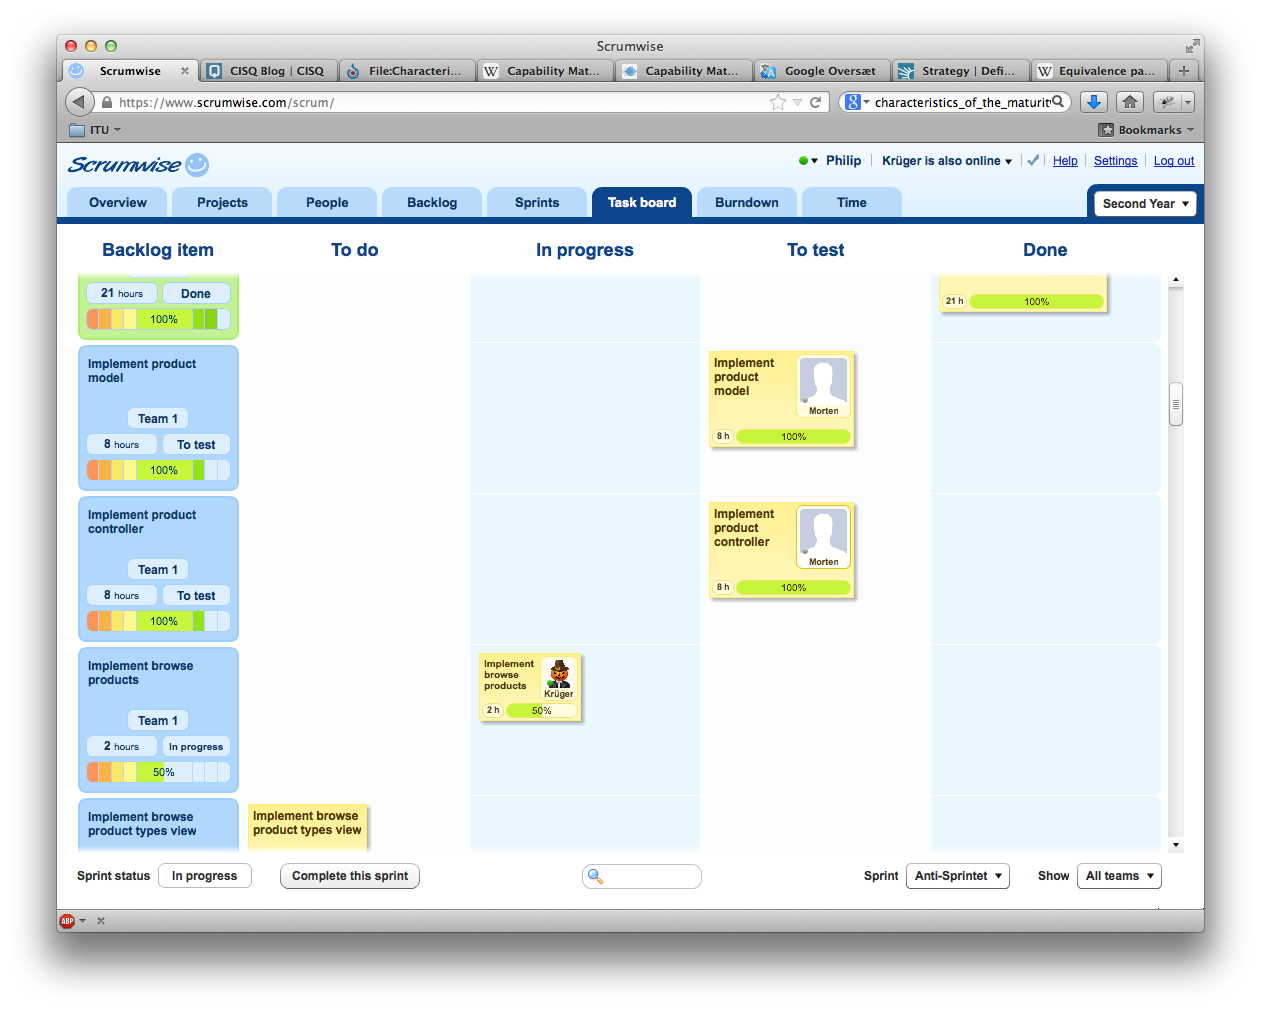
\includegraphics[width=\textwidth]{illustrations/taskboard}
  \caption{Taskboard.}
  \label{taskboard}
\end{figure}

\begin{figure}[H]
  \centering
  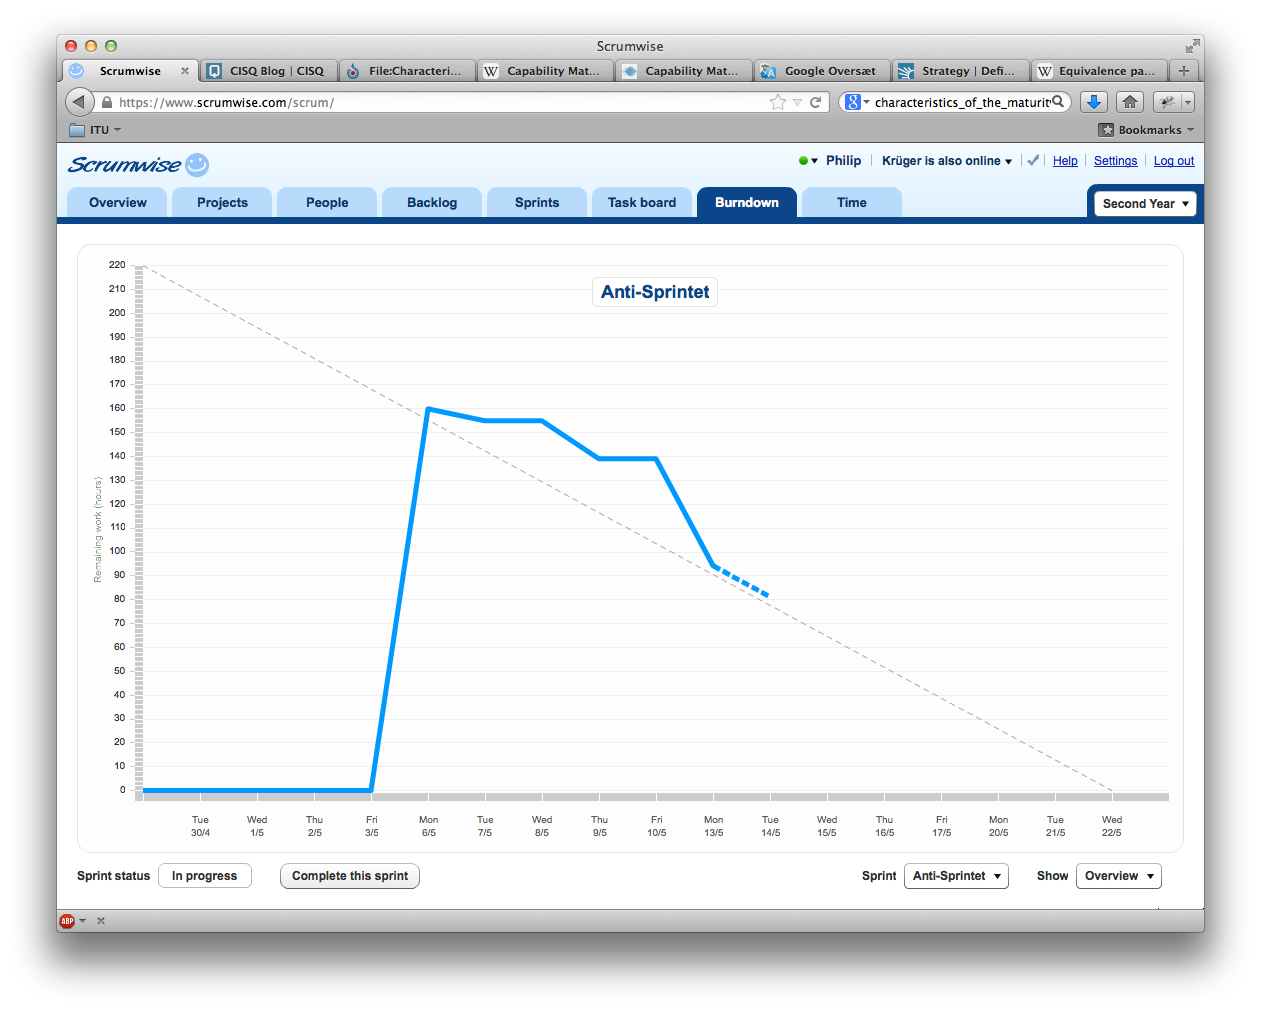
\includegraphics[width=\textwidth]{illustrations/burndown}
  \caption{Burndown chart. At the point of writing it seems like we are on track.}
  \label{burndown}
\end{figure}

% BACKLOG TABLE START %
\begin{longtable}{|p{200px}|p{200px}|}
\caption[Backlog]{Backlog} \label{backlog} \\

\hline \multicolumn{1}{|c|}{\textbf{Time (s)}} & \multicolumn{1}{c|}{\textbf{Description}} \\
\endfirsthead

\multicolumn{2}{c}%
{{\bfseries \tablename\ \thetable{} -- continued from previous page}} \\
\hline \multicolumn{1}{|c|}{\textbf{Name (s)}} &
\multicolumn{1}{c|}{\textbf{Description}} \\ \hline 
\endhead

\hline %\multicolumn{3}{|r|}{{Continued on next page}} \\ \hline
\endfoot

\hline
\endlastfoot
    \hline
	Convert API images to spreadsheet & ~  \\
	\hline
		Create diagrams & Class diagrams, SSD, Design mockups (if time), Package diagram, etc. \\ \hline
	Program structure & Create repository, files and empty methods from the interface \\ \hline
	Implement composite structure base classes & ~ \\ \hline
	Implement JSON class & ~  \\ \hline
	Implement web-service class & ~ \\ \hline
	Implement page view & ~  \\ \hline
	Implement base functionality for views & Slide out, Click field to edit, Fixed header, Ajax mouseover to view, Buttons, Fields,	etc. \\ \hline
	Implement product model & ~  \\ \hline
	Implement product controller & ~  \\ \hline
	Implement browse products & ~  \\ \hline
	Implement browse product types view & ~  \\
	Implement auth model & ~  \\ \hline
	Implement auth controller & ~  \\ \hline
	Implement login/create widget in header & ~  \\ \hline
	Implement logged-in mouseover in header view & ~  \\ \hline	
	Implement single dropdown autocomplete widget & ~  \\ \hline
	Implement multiple dropdown autocomplete widget & ~  \\ \hline
	Implement product view & ~  \\ \hline
	Implement rating widget view & ~  \\ \hline
	Implement purchases model & ~  \\ \hline
	Implement purchases controller & ~  \\ \hline
	Implement buy/rent widget view & ~  \\ \hline
	Implement stream view & ~  \\ \hline
	Implement credits model & ~  \\ \hline
	Implement credits controller & ~  \\ \hline
	Implement account model & ~  \\ \hline
	Implement account controller & ~  \\ \hline
	Implement account profile view & ~  \\ \hline
	Implement purchases view & ~  \\ \hline
	Implement customer dashboard view & ~  \\ \hline
	Implement content provider dashboard view & ~  \\ \hline
	Implement search products view & ~  \\ \hline
	Implement browse accounts view & ~  \\ 
	Test WCF Service Controllers & Helper Classes needs to be refactored to use interfaces. Mockup implementations needs to be made. \\ \hline
	Define Report Structure & ~  \\ \hline
	Write Introduction & ~  \\ \hline
	Write Problem statement and requirements & ~  \\ \hline
	Write Use Cases & Server and client  \\ \hline
	Write Software Analysis (server) & Why have we chosen the technologies we have? \\ \hline
	Write Software Design and architecture (server) & ~  \\ \hline
	Write Testing (server) & ~  \\ \hline
	Write Software Analysis (client) & ~  \\ \hline
	Write Software Design and architecture (client) & ~  \\ \hline
	Write Testing (client) & ~  \\ \hline
	Write Conclusion & ~  \\ \hline
	Write Abstract & ~  \\ \hline
\end{longtable}
\newpage

\begin{landscape}
\begin{figure}[H]
  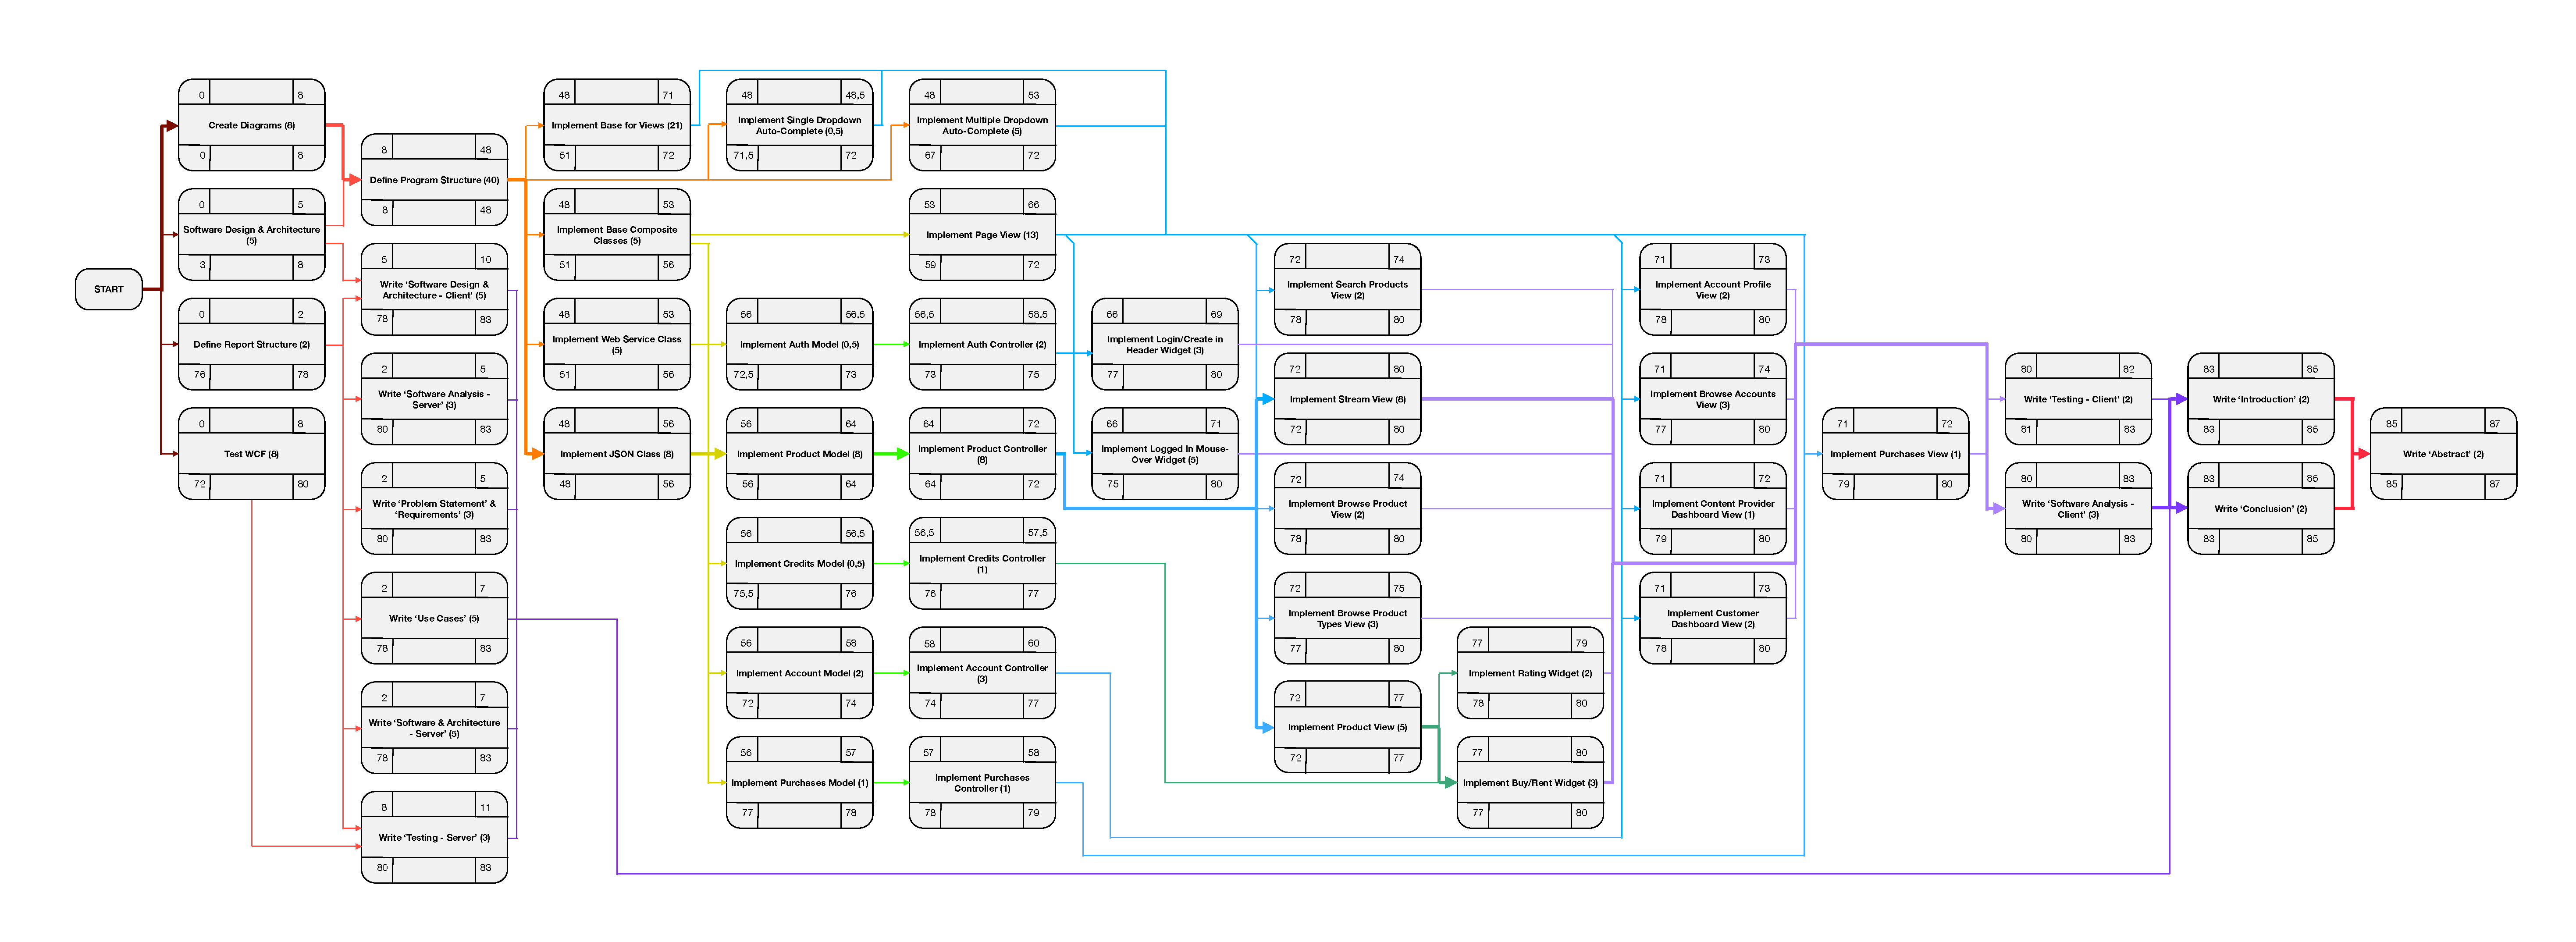
\includepdf[landscape]{illustrations/Dependency_network.pdf}
  \caption{Dependency network}
  \label{dependency_network}
\end{figure}
\end{landscape}

\newpage
\renewcommand{\section}[2]{} % Removing some bug where it added a heading after this? :S

% Add bibliography
\bibliographystyle{cell}
\bibliography{bib}
\end{document}